\chapter{Implementation} \label{Implementation}

	This chapter delves into the implementation of the planned architecture defined in section \ref{archdecision}.
	First I will introduce the starting point of the project.
	Then I will go into detail about the implementation of a client within the backend, which communicates with 
	the generator microservice. Finally I will go into detail
	regarding the inner workings of the generator server.

	The starting backend's class diagram can be found in the appendix at \ref{startingbackenduml}.
	The implemented generator client can be seen at \ref{backendclientuml}.
	The implemented generator microservice can be seen at \ref{generatorserveruml}.

	\section{Starting point} \label{Starting point}
		First, I will introduce the starting point of the project, so we get an overview, of how the backend initially worked regarding the model
		generations.

		The PushServiceDispatcher is the class responsible for calling the functions of the ModelGenerationService instance, and thus initiating
		the generation related methods.

		\subsection{ModelGenerationService} \label{ModelGenerationService}
			The \textit{ModelGenerationService} is a core component of the application, designed to handle the starting and management of
			model generation workers (section \ref{ModelGenerationWorker}) on the backend server. 
			It is a singleton class, so from a generator point of view, we might consider this class to be the real dispatcher.

			The key features and responsibilities of the class include:
			\begin{itemize}
				\item{\textbf{Service Initialization:}} The \textit{ModelGenerationService} is a singleton, 
				ensuring a single, consistent instance throughout the application's lifecycle.
				It retrieves configuration parameters such as the model generation timeout 
				from the environment, defaulting to 600 seconds if not explicitly set.
				\item{\textbf{Model Generation Workflow:}} The main responsibility of the service is to execute model generation requests 
				by instantiating workers (\textit{ModelGenerationWorker}), using multithreading. The amount of threads 
				where the workers can be run is set via an environment variable (REFINERY\_MODEL\_GENERATION\_THREAD\_COUNT 
				\cite{generationthread}).

				The service interacts with the document’s \textit{ModelGenerationManager} to monitor the workers.
				The timeout and cancellation is handled via the use of cancelation tokens.
			\end{itemize}
			The use of dependency injection for worker provisioning ensures that the service is decoupled from the specific implementation details
			of task execution, making it easier to extend or modify in the future.

		\subsection{ModelGenerationWorker} \label{ModelGenerationWorker}
			The \textit{ModelGenerationWorker} class is where the actual model generations happen. 
			It operates as an independent thread, processing generation requests in a thread-safe and scalable manner. 
			Its multithreaded design uses Java's ExecutorService to manage task execution efficiently within a threadpool.

			Each worker instance is uniquely identified by their UUID. Before execution, the worker’s state is configured 
			with essential inputs, such as the document containing the generation request, a random seed, and a timeout value. 
			This sets up the generation and prepares the worker for execution.

			The worker’s primary responsibility is to handle the computational workflow, 
			which includes parsing the input into a formal problem, generating a solution, extracting metadata, 
			and converting results into a JSON (section \ref{backgrjson}) format. 
			Throughout this process, the worker monitors for cancellation requests and timeout. 

			Once a task is completed, the worker notifies the service whether the generation was successful or ran into an error. 

	\section{Generator Client} \label{Generator Client}
			Now that the deployed implementation has been been described, we can restructure our application, so that the 
			model generation is done via the generation microservice.

			The design of the \textit{ModelGenerationService} (section \ref{ModelGenerationService}) is scalable and modular:
			By delegating the actual computation to workers (ModelGenerationWorker, section \ref{ModelGenerationWorker}), 
			the service separates dispatching and execution. 
			
			This comes in handy, when implementing our client for communication with
			the generator server. We have to implement a client, which communicates generation requests towards the generator server,
			and upon completion, receives such generation results.

			The implemented client's UML class diagram, alongside the modifications to the backend can be seen in appendix \ref{backendclientuml}.

			\subsection{GeneratorWebSocketEndpoint} \label{GeneratorWebSocketEndpoint}
				This class is responsible for sending generation requests and handling responses is implemented as the 
				GeneratorWebSocketEndpoint class,
				using Jetty's WebSocket API (section \ref{backgrjetty}). 
				This endpoint facilitates asynchronous communication with the generator microservice, 
				ensuring efficient request management over WebSocket connections. 

			In the following sections, I will describe the key responsibilities and functionalities of the GeneratorWebSocketEndpoint class.
			\subsubsection{WebSocket Configuration} 
				The server, which the client is communicating with, can be configured.
				\begin{itemize}
					\item The WebSocket URI is dynamically determined based on environment variables (\textit{REFINERY\_GENERATOR\_WS\_HOST} 
					and \textit{REFINERY\_GENERATOR\_WS\_PORT}). If these are unset, default values (localhost and 1314) are used to ensure flexibility during deployment.
					\item The constructor initializes a WebSocketClient instance and sets default values, such as the worker's UUID and timeout duration.
				\end{itemize} 
			\subsubsection{Communication towards the server} 
				\begin{itemize}
					\item The client connects to the server via a ClientUpgradeRequest. The connection includes a custom header for the UUID of the worker.
					\item Sending the generation requests via sendGenerationRequest method. The method sends a structured JSON payload containing the request type,
					the UUID, the problem description, and a random seed. This start the model generation process on the server
					\item \label{clientcancel}Sending generation cancel requests via the sendCancelRequest method. This client sends a JSON, with the UUID of the generation to be 
					executed. Each generation opens a new session, with a new UUID for the server, so they can be uniquely idenfitied.
				\end{itemize} 
			\subsubsection{Receiving from the server} 
				Responses from the server are handled by the onText method, which processes various types of messages 
				(result, error, nodesMetadata, relationsMetadata, partialInterpretation), parsing them into appropriate data 
				structures and queuing them for consumption in their appropiate result queues (section \ref{resultqueues}).

			\subsubsection{Parsing responses from the queue} \label{resultqueues}
				The client maintains several LinkedBlockingQueue instances to manage received data:
				\begin{itemize}
					\item responseQueue: Stores results or errors associated with the generation process.
					\item nodesMetaDataQueue: Holds metadata about nodes in the generated model.
					\item relationsMetadataQueue: Queues relation metadata details.
					\item partialInterpretationQueue: Handles intermediate model interpretation data.
				\end{itemize} 
				The queues are accessed with timeout constraints to prevent indefinite blocking during retrieval. The timeout is set up by the class'
				timeout variable. 
				
				The LinkedBlockingQueue allowed the onText method, to put the received generation
				results into the queue, while the client is waiting for the results to arrive from the server. As soon as an element is put into the queue
				it can be popped from it. This way our code is safely waiting for the results
				to arrive from the server and no concurrency issues can arise. As I have already mentioned, each generation request instantiates a new
				client, so the size of these queues can only be between 0 and 1. No other generation client is accessing these queues of the instances.


		\subsection{ModelRemoteGenerationWorker} \label{ModelRemoteGenerationWorker}
			\subsubsection{Core functionality}
				The ModelRemoteGenerationWorker manages the WebSocket client (section \ref{GeneratorWebSocketEndpoint}) in a multithreaded
				fashion. The class operates with the same threadpool introduced in section \ref{ModelGenerationWorker}. This way, the old 
				local generation (section \ref{ModelGenerationWorker}) could be replaced with this remote client, 
				with no other major changes done to the codebase.

			\subsubsection{IGenerationWorker}
				For implementation, the IGenerationWorker interface was created, which defines a unified API for all generation workers. 
				This interface standardizes the core operations, including task initialization, execution, timeout management, and cancellation.
				This abstraction ensures that the backend can switch between local and remote workers. The switch can be toggled via
				an environment variable. The old ModelGenerationWorker and the ModelRemoteGenerationWorker both implement this interface.

				The key methods from the interface include:
				\begin{itemize}
					\item setState: Configures the worker with the input document, random seed, and timeout settings.
					\item start and startTimeout: Enqueues the worker for execution and schedules a timeout to enforce task completion within a defined duration.
					\item doRun: Executes the remote model generation logic by communicating with the external service.
					\item \label{workercancel}cancel: Cancels the task, ensuring both local and remote operations are halted gracefully.
				\end{itemize}

			\subsubsection{Workflow}
				The execution process of ModelRemoteGenerationWorker begins with setup and state configuration. 

				During task execution, the worker sends a generation request to the remote service by using a WebSocket client instance (GeneratorWebSocketEndpoint). 
				The server's responses are processed incrementally.

				The task completes successfully upon retrieving all necessary results, or it is terminated on errors, cancellation, or timeout.

				Timeouts and cancellations are managed via a ScheduledExecutorService, ensuring that the system remains responsive and resources are freed promptly. In case of errors, the worker captures exceptions, logs the issues, and notifies the backend with appropriate error results.

				The interaction between the GeneratorWebSocketEndpoint and the ModelRemoteGenerationWorker 
				showcases how client-side operations are integrated into the existing codebase.

	\section{Generator Server} \label{Generator Server}
		Now that the client side of the generation process has been introduced, the server side implementation is what should be described next.
		The main idea behind this implementation, was to take the experiences of the local model generation worker, and basically implement everything that 
		is necessary for a generation to happen, in a multithreaded way, on our microservice. It is basically the implementation of 
		the ModelGenerationWorker (section \ref{ModelGenerationWorker}) on a separate server.

		The UML class diagram of the Generator Server can be found in the Appendix at \ref{generatorserveruml}.

		\subsection{GeneratorServerEndpoint} \label{GeneratorServerEndpoint}
			The GeneratorServerEndpoint is a WebSocket server endpoint utilizing Jetty's WebSocket server API \ref{backgrjetty}. 
			The server actively listens
			to generation requests and upon receiving submits the requests to the ModelGeneratorDispatcher 
			(section \ref{ModelGeneratorDispatcher}).

			\subsubsection{Core Functionality} \label{Core Functionality}
				The two most important functionalities of the class are the handling of the generation requests and cancelation requests, which are
				 received over the 
				WebSocket sessions. 
				
				When a message of type "generationRequest" is received, the endpoint extracts generation details 
				such as the unique identifier (UUID), random seed, and problem description. The data is sent by the client (section \ref{GeneratorWebSocketEndpoint} 
				and section \ref{ModelRemoteGenerationWorker}) via JSON, so extracting the
				needed key-value pairs is straighforward. These are then forwarded to the ModelGeneratorDispatcher, 
				which manages the actual model generation task.

				\label{serverendpointcancel}For "cancel" messages, the endpoint instructs the ModelGeneratorDispatcher to cancel an ongoing generation task associated with the provided uuid.

				Any errors during the WebSocket communication are captured, logged.

				When a WebSocket session is closed, the endpoint notifies the ModelGeneratorDispatcher to clean up resources associated with the disconnected client.

			\subsubsection{Integration into the workflow} \label{Integration into the workflow}
				The GeneratorServerEndpoint serves as the entry point for remote clients into the generator microservice. 
				It relies on the ModelGeneratorDispatcher to manage generation and cancellation tasks. This provides a clean separation of concerns. 
				The design ensures that the endpoint focuses solely on communication, while the dispatcher handles the generation tasks.

			\subsubsection{Scalability and Extensibility} \label{Scalability and Extensibility}
				This WebSocket-based implementation allows the backend to support multiple concurrent client connections efficiently. 
				By using asynchronous communication, it ensures that tasks are queued and processed without blocking the ongoing generations. 
				The modular design makes it easy to extend functionality, such as adding new message types or enhancing error handling mechanisms.


		\subsection{ModelGeneratorDispatcher} \label{ModelGeneratorDispatcher}
			The ModelGeneratorDispatcher is a singleton class designed to manage and execute model generation requests on separate threads. 
			Its primary role is to coordinate the model generation tasks, making sure that they run concurrently. 
			This dispatcher simplifies the handling of multiple requests 
			and helps with maintaining system consistency.

			\subsubsection{Key features} \label{Key features}
			The class implements the singleton design pattern to guarantee that only one instance of ModelGeneratorDispatcher exists throughout the application. 
			This is achieved via the use of a private constructor which prevents instantiation of the class from the outside, ensuring 
			that all interactions go through the singleton instance.
			This provides centralized control and avoids conflicting task management.

			The GeneratorServerEndpoint submits the received generation requests for this class. 
			Each model generation request is executed in a separate thread. 
			This is achieved through the ModelGeneratorExecutor (section \ref{ModelGenerationExecutor}) class, which handles the task logic.
			The running model generations (ModelGenerationExecutor) are stored in a hashmap. The processing threads are identified by 
			the UUID of the generation in the hashmap.

			\label{servercanceldispatcher}Ongoing tasks can be cancelled via the UUID of the generation. As the hashmap stores these generation tasks identified by their UUID, it is fairly easy to do so.

			Once a client has disconnected, the belonging task is cancelled, if not finished yet. The said task is removed from the hashmap. The UUID identification is 
			useful here aswell.

		\subsection{ModelGeneratorExecutor}\label{ModelGenerationExecutor}
		The ModelGeneratorExecutor is a class responsible for performing the actual model generation tasks. It runs on a separate thread, 
		making it suitable for concurrent processing. This class does what the original ModelGenerationWorker 
		(section \ref{ModelGenerationWorker}) did in the original implementation. 
		It even operates as part of a dispatcher system. The running of these executor threads is started by the ModelGeneratorDispatcher 
		(section \ref{ModelGeneratorDispatcher}).

		\subsubsection{Key features and responsibilities}\label{Key features and responsibilites}
			The main responsibilites of the class are the following:
			\begin{itemize}
				\item \textbf{Initialization:} Before starting, it initializes the problem by loading the problem description, random seed, and WebSocket session details. These were
				received by the GeneratorServerEndpoint over WebSocket, and are given to an executor object by the ModelGeneratorDispatcher.
				\item \textbf{Task Execution:} The class handles the execution of the model generation. This is done in the exact same way, as it was done previously at the local ModelGenerationWorker.
				\item \textbf{Client communication:} By receiving an open WebSocket session in the constructor, the class instance can send generation 
				state results, metadata and errors to the clients.
				\item \label{serverexecutorcancel}\textbf{Cancellation support:}The task can be interrupted or canceled at any point, 
				making sure that unnecessary processing is avoided. This is especially useful for timeout scenarios or user-initiated cancellations.
			\end{itemize}

		\subsection{ServerLauncher}\label{Serverlauncher}
		The ServerLauncher class serves as the entry point for starting a WebSocket server that 
		processes model generation requests (section \ref{GeneratorServerEndpoint}). It listens on a configurable port, defaulting to 1314 
		unless overridden by the \textit{REFINERY\_GENERATOR\_WS\_PORT} environment variable. 
		
		The class sets up a Jetty server, running the implemented GeneratorServerEndpoint.
		Once everything is configured, the server is started to handle incoming requests. 
		This class essentially establishes the server infrastructure for the application.

	\section{Containerization}\label{Containerization}
		The new generator microservice was added 
		to the "run" task of the backend gradle project, and as such, the workings of the application could be tested locally in a manual fashion. 
		
		Containerization (\ref{backgcontainer}) was the next step in 
		updating our application. 

		Even before the restructuring, the build pipeline already existed. My main task was integrating the generator server docker image creation
		into these available scripts of the pipeline. 

		\subsection{Preparation scripts}\label{Preparation scripts}
			The process begins with a build script that compiles the project's distributed components, such as the backend and generator microservices, into portable archives. 
			This is done via the use of Gradle (\ref{backgrgradle}).

			One script organizes and optimizes the build outputs, ensuring shared dependencies are deduplicated and arranged for efficient reuse. 
			It also prepares architecture-specific resources to support multi-architecture Docker builds, arranging all necessary files into a structured context for image creation.
			I had to modify this script, so that it also handles the same process for the newly created generator server's (\ref{Generator Server}) archives.

			Finally, a dedicated script builds and optionally pushes Docker images using a multi-stage build configuration. 
			This configuration leverages tools like Docker Buildx and supports deployment across different architectures, ensuring compatibility. 

		\subsection{Docker images}\label{Docker images}
			The project utilizes a structured and reusable approach to Docker (\ref{backgdocker}) image creation, leveraging a common base image and architecture-specific 
			optimizations to support multi-architecture compatibility.

			A configuration file specifies the group of targets (like the base, backend and generator) and individual build configurations for each target. 
			These targets are the created docker images.

			These targets share a lightweight base image that includes essential runtime dependencies. 
			Each target builds on this foundation, adding service-specific layers such as dependencies, binaries, and configuration files.

			I implemented the Dockerfile.generator to containerize the generator service efficiently. It builds the service using a multi-stage process, 
			layering runtime dependencies, application files, and configuration (like environment variables and exposed ports). 
			It uses the base image as its starting point.

			I also created a Docker Compose (\ref{backgdockercompose}) file for the local deployment of the application. Via this, the manual testing of the 
			created application docker images can be done. Before deploying to the production infrastructure, this can add an extra layer of ensuring proper workings.

			The finished images were pushed to the Docker Hub registry. The public repository containing the images (backend,
			generator) can be accessible by anyone, and are needed for the AWS deployment.


	\section{Deploying on AWS} \label{awsdeploy}
		In this section I will describe the deployment of the modified Refinery backend and the Generator microservice. The deployment will be 
		done according to the plan setup in \ref{awsdecision}.

		I registered a new AWS account with my own private email address.
		For the creation of the infrastructure I used the AWS Management Console, which is the web GUI for 
		managing our AWS infrastructure.

		\subsection{Task definitions} \label{awstasks}
			First I set my tasks up. The tasks are basically the container instances of an application within the AWS ECS environment. 
			I created a task
			for the generator microservice called refinery-generator and the backend server called refinery-language-web.
			In the task configuration, I set the tasks to run on EC2 instances, provided the belonging docker registry link for the service,
			assigned the port mappings for the appropiate listening ports, and set the environment variables, 
			such as the generation host and port. The refinery-language-web task definition needed the "REFINERY\_GENERATOR\_WS\_HOST" to 
			be equal to the load balancer of the generator microservice's load balancer (this had several issues as explained 
			in section \ref{ALB NAT}).
			I set the networking mode for both tasks to be awsvpc, as they would be deployed on the same Virtual Private Cloud.
			Health checks also had to be implemented, so that our service knows, that the application is running and is in a stable state.
			For health checks, I used basic curl requests to the host and ports of the services. This needed modification for 
			the generator server codebase (section \ref{healthcheck}).

		\subsection{Service definitions} \label{awsservices}
			I created a refinery cluster, with services running the defined tasks in \ref{awstasks}. The services are within an 
			EC2 auto scaling group. 
			This allows us to scale our container instances, if they are heavily used and the resource usage is over a threshold.
			For this I set up two treshholds:
			\begin{itemize}
				\item CPU usage: If the average CPU usage is over 70\% for more than 300 seconds, a new instance is deployed.
				\item Memory usage: If the average RAM usage is over 70\% for more than 300 seconds, a new instance is deployed.
			\end{itemize}
			I used Amazon's t3.micro EC2 instances for the auto scaling group, which are eligible for the free tier accounts. 
			They each have 2 vCPUs with 4 threads and 1GB of RAM.
		
		\subsection{Load Balancer definition} \label{awslb}
			An application load balancer (ALB) was created for the 
			backend and the generator server. The ALB would forward traffic to the running container instances within a target group, as longs as their
			health checks pass. 
			The ALB would be reachable for anyone on the internet on port 80. This port forwards traffic to the target group of the backend of the application.
			On port 81, the forwarding of the generator microservice requests is done towards the generator target group. However, this port is configured
			to accept requests only within the security group of the application. As such, only the backend can send requests to the microservice, hiding it 
			away from the public internet.
			I set the load balancing algorithm to the default round-robin, but least-used can also be a viable option.

	\section{Challenges during the implementation} \label{challenges}
	\subsection{Resource usage of development}
		I wanted to develop on the Linux operating system, via the use of Windows Subsystem for Linux (WSL). WSL was needed because 
		of the build scripts, which were implemented for UNIX shells.

		When I initially opened the Refinery gradle project via a remote connection to my WSL the resource usage 
		for the gradle project indexing was huge. The 8-core Ryzen 7 CPU was sitting at around 70\%  usage, alongside 
		16 gigabytes of my system memory being 92-99\% occupied. 
		
		The initial indexing of the Gradle project took around 45-60 minutes. Even upon completion the resource usages did not improve. 
		The same amount of RAM
		was used by the WSL and it would not become lower. 

		\begin{figure}[h!]
			\begin{center}
				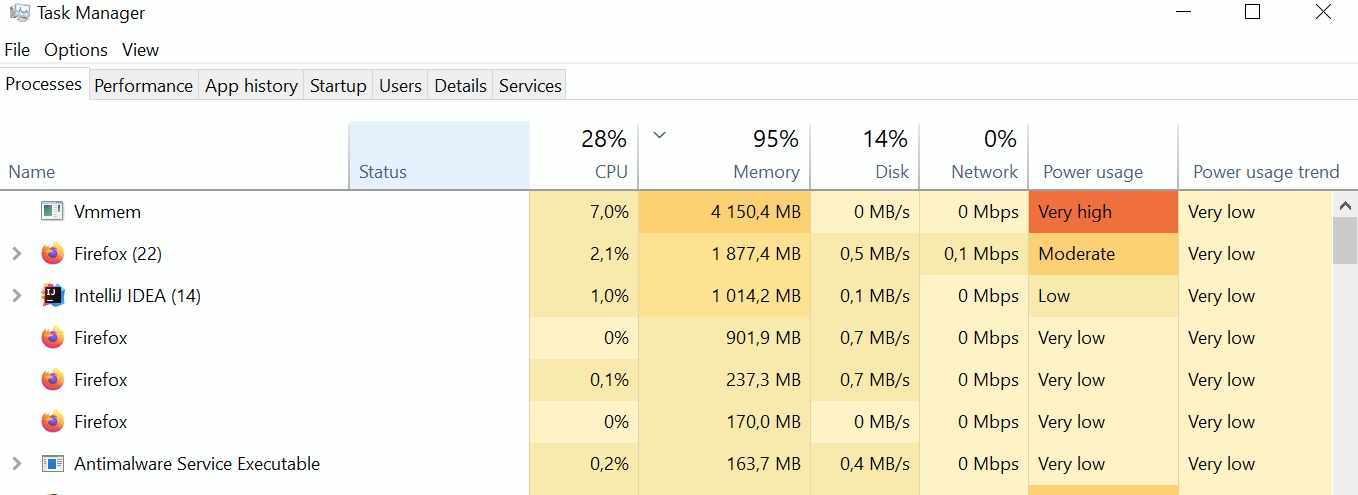
\includegraphics[scale=0.35]{include/imgs/res_usage.jpg}
				\caption{Resource usage during developing on WSL}
				\label{resourceusagewsl}
			\end{center}
		\end{figure}

		As a result of this, I have given up on the development using WSL. I developed the application on Windows, while using WSL only for the
		dockerization (\ref{Containerization}) of the finished applications.

	\subsection{Deduplication for docker images}
		The initial context preparation in section \ref{Preparation scripts} was implemented for two different distributions (the basic backend 
		named web, and a generator cli called cli). The common\_libs creation for both of these distributed images was straightforward
		as the two distributions only had limited amount of JARs that they both used.

		With my project, a new distribution for the generator server was created. Originally I wanted to implement the deduplication in a way,
		where if two of the three distributions contained a JAR, the JAR would be put in the common\_libs folder.
		However, this implementation did not seem useful. In this case all of the resources needed for the web distribution were added to the common folder.
		As such, the shell script would have needed to be modified aswell, so that it could handle empty dist folders during the pipeline. 
		On the other hand
		all of the files from the common library would be put in the base docker image, even tho it might not be needed for the 
		running of our application. This would risk the bloating of the base image.

		I decided to add only those resources to the common library, which are used in all of the created docker images. 
		As a result, the base image is not bloated and the shell script did not need many modifications.

	\subsection{Health check for the generator server} \label{healthcheck}
		When deploying an application with the use of an Application Load Balancer, a target group of the tasks has to be specified.
		The load balancer needs to keep track of the running task docker container instances, so that it can decide, whether requests can be 
		forwarded to the running microservice. A health check has to be put in use, so that the load balancer can register the running instances.

		In my implementation of the generator server at section \ref{GeneratorServerEndpoint}, I only created a WebSocket server. However, Jetty 
		WebSocket servers won't respond to regular HTTP requests. With this original implementation, the health check for the load balancer would
		not work: it always signaled that the task was not running, as it wouldn't respond to the curl http requests towards the default path (/).

		As a workaround, I created a servlet called HealthCheckServlet, which responds to HTTP get requests (section \ref{backgrhttp}) at the path "/healthcheck",
		by returning a "Server works!" plain text.

		I added the servlet to the ServerLauncher of the generator microservice. By this, the load balancer can ensure the healthy state of the 
		the server instances, by sending a curl request to the "/healthcheck" path of the generator server.

	\subsection{Application Load Balancer and NAT} \label{ALB NAT}
		During the deployment process, I faced persistent issues with the backend failing to connect to the generator microservice 
		through the Application Load Balancer (ALB), resulting in request timeouts. Initially, I suspected an Access Control List (ACL) 
		issue within the VPC hosting the infrastructure. To rule this out, I configured the ACL to allow all inbound and outbound traffic 
		and ensured Security Group policies were set to restrict access to the generator microservice only from the backend server. 
		Despite these changes, the issue persisted, with the backend unable to connect to the ALB's DNS.

		To further investigate, I accessed the EC2 instances running the ECS tasks by configuring an SSH key pair. 
		Using tools like curl and ping, I confirmed the EC2 instance could communicate with the ALB, including receiving expected responses 
		from the generator microservice's health check endpoint (\ref{healthcheck}). However, when testing connectivity from within the container 
		using a statically compiled curl binary, no response was received from the ALB.

		Through further research, I identified the root cause: ECS tasks using the awsvpc network mode are assigned private IP addresses, 
		while the ALB has only a public IP address. Since AWS does not perform Network Address Translation (NAT) within the VPC, 
		the ECS tasks could not directly reach the public ALB. This required implementing a solution to perform the necessary address translation, 
		ensuring proper communication between the backend and the generator microservice.

		\begin{figure}[h!]
			\begin{center}
				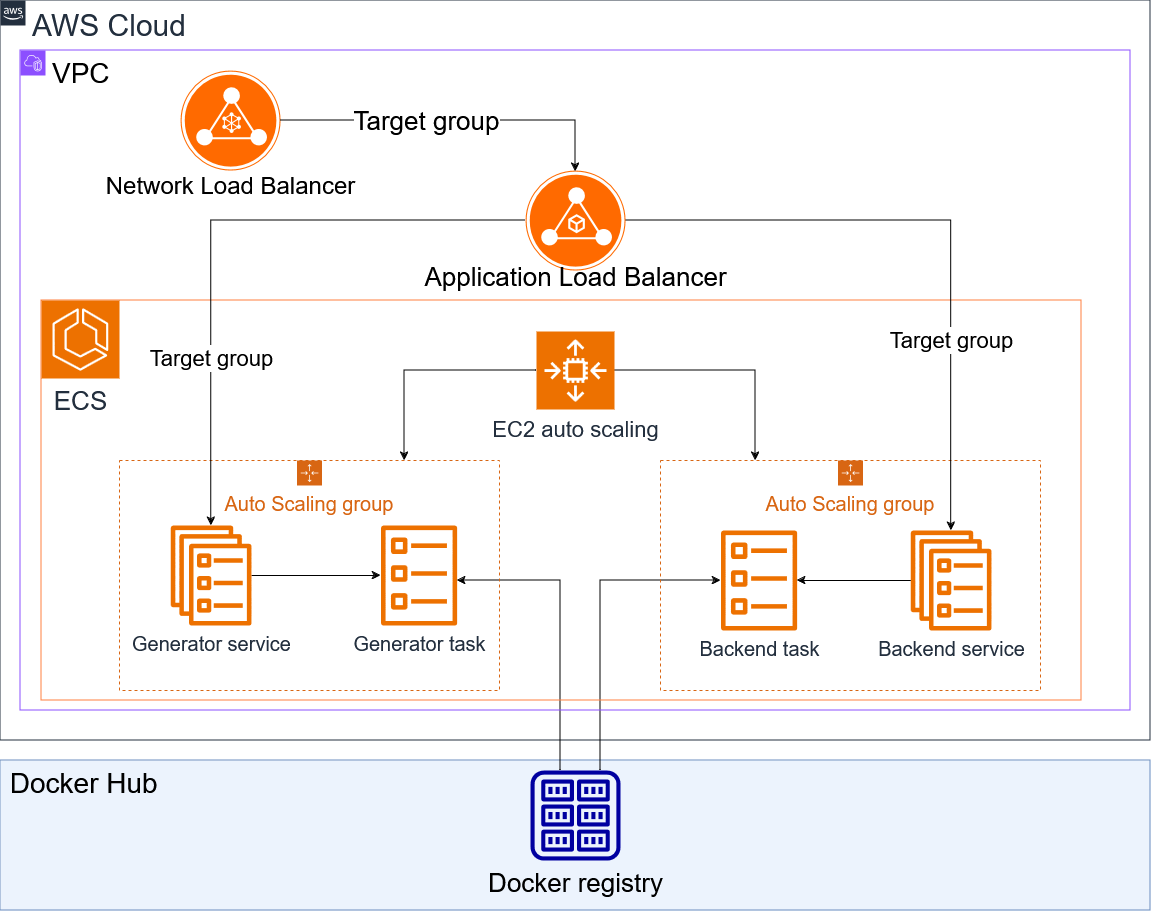
\includegraphics[scale=0.35]{include/imgs/final_aws_infra.png}
				\caption{Final deployed infrastructure}
				\label{infrafinal}
			\end{center}
		\end{figure}

		I faced two options to address the public-private IP connectivity issue: setting up a Network Load Balancer (NLB) or a Network Address Translation (NAT) gateway.

		The NLB, like the ALB, operates using target groups but supports private IPv4 addresses. 
		By configuring the NLB to use the ALB’s public IP as a target, the NLB effectively serves as a NAT solution, enabling private ECS tasks to communicate with the ALB. 
		Alternatively, the NAT gateway would facilitate communication between services across public and private subnets and provide greater flexibility 
		for future infrastructure expansions, even outside AWS.

		I chose the NLB due to its lower cost. The NAT gateway has a fixed hourly rate of \$0.046 (\cite{natprice}), whereas the NLB’s cost is traffic-dependent (\cite{nlbprice}). 
		Based on AWS’s pricing examples, the NLB was projected to cost nearly half as much under lower traffic conditions. 
		To finalize the setup, I updated the backend task configuration to point the REFINERY\_GENERATOR\_WS\_HOST environment variable to the NLB's DNS. 
		The completed infrastructure setup is illustrated in Figure \ref{infrafinal}.